\documentclass[a4paper, 12pt]{article}
\usepackage{geometry}
\geometry{a4paper,
total={170mm,257mm},left=2cm,right=2cm,
top=2cm,bottom=2cm}

\usepackage{mathtext}
\usepackage{amsmath}
\usepackage[T2A]{fontenc}
\usepackage[utf8]{inputenc}
\usepackage[english,russian]{babel}
\usepackage{graphicx, float}
\usepackage{tabularx, colortbl}
\usepackage{caption}
\captionsetup{labelsep=period}

\newcommand{\parag}[1]{\paragraph*{#1:}}
\DeclareSymbolFont{T2Aletters}{T2A}{cmr}{m}{it}
\newcounter{Points}
\setcounter{Points}{1}
\newcommand{\point}{\arabic{Points}. \addtocounter{Points}{1}}
\newcolumntype{C}{>{\centering\arraybackslash}X}

\author{Калинин Даниил, Б01-110}
\date{\today}
\title{Лабораторная работа 4.1.2. Моделирование оптических приборов и определение их увеличения}

\begin{document}
\maketitle
\parindent=0cm

\parag {Цель работы}
Определить фокусные расстояния собирающих и рассеивающих линз, смоделировать ход лучей в трубе Галилея, трубе Кеплера и микроскопе, определить их увеличение.

\parag {В работе используются}
Оптическая скамья, набор линз, экран, осветитель со шкалой, зрительная труба, диафрагма, линейка.

\parag {Ход работы} ~\\
\point Для начала определим примерные фокусные расстояния линз. Для этого возьмем парралельный пучок лучей и будем добиваться четкого изображения, если изображения наблюдаться не будет, то линза -- рассеивающая. Проделаем такой эксперимент со всеми линзами. Результат занесем в таблицу  \ref{tabl:approx_focuses}.

\begin{table}[h]
    \centering
    \begin{tabular}{|c|c|}
    \hline 
        Номер линзы & Приблизительное фокусное расстояние, см. \\ \hline
        1 &  7.7      \\ \hline
        2 &  10       \\ \hline
        3 &  20.7     \\ \hline
        4 &  31       \\ \hline
        5 &  --       \\ \hline
        
    \end{tabular}
    \caption{Приблизительные фокусные расстояния линз}
    \label{tabl:approx_focuses}
\end{table}

Таким образом, у нас получилось, что линзы 1-4 -- собирающие, а линза 5 -- рассеивающая.

\point Теперь определим точное фокусное расстояние собирающий линз. Для этого сначала настроим зрительную трубу на бесконечность, а затем будем располагать линзы на расстоянии, примерно равном фокуснуму. Передвигая линзу вдоль скамьи, получим в окуляре зрительной трубы четкое изображение предмета -- миллиметровой сетки, тогда расстояние между предметом и серединой линзы равно фокуснуму. Полученные измерения занесем в таблицу \ref{tabl:collecting_preciese_focuses}. 

\begin{table}[h]
    \centering
    \begin{tabular}{|c|c|}
    \hline 
        Номер линзы & Фокусное расстояние, см. \\ \hline
        1 &  7.5        \\ \hline
        2 &  10.6       \\ \hline
        3 &  19.3       \\ \hline
        4 &  28.1       \\ \hline
        
    \end{tabular}
    \caption{Фокусные расстояния собирающих линз}
    \label{tabl:collecting_preciese_focuses}
\end{table}

\point Далее определим фокусное расстояние рассеивающей линзы. Для начала, получим увеличенное изображение сетки при помощи короткофокусной линзы № 1. Измерим расстояние между линзой и экраном: $a_0 = 37.5~ см.$ Сразу за экраном разместим зрительную трубу, настроенную на бесконечность, уберем экран, а на его месте поставим рассеивающую линзу. (Установка изображена на рисунке \ref{img:scatter_lens}). 

\begin{figure}[h]
    \centering
    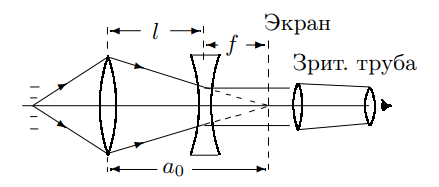
\includegraphics[scale=0.7]{minus_lens.png}
    \caption{Схема эксперимента по измерению фокусного расстояния рассеивающей линзы.}
    \label{img:scatter_lens}
\end{figure}

Перемещая рассеивающую линзу, добьемся четкого изображения сетки в зрительной трубе. Измерив расстояние между линзами, расчитаем фокусное расстояние рассеивающей линзы: $l = 11.5 ~ см. $, $f_5 = a_0 - l = 26 ~ см.$

\point Измерив фокусные расстояния, приступим к моделированию оптических приборов. Первым смоделериуем трубу Кеплера. 

Ход лучей в трубе Кеплера представлен на рисунке \ref{img:rays_way_kepler}. Пользуясь рисунком, найдем теоретическое увеличение системы.

\begin{figure}[h]
    \centering
    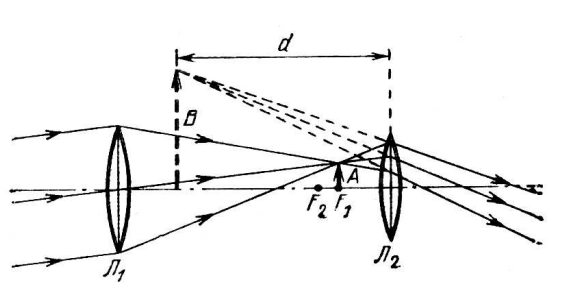
\includegraphics[scale=0.7]{kepler.png}
    \caption{Ход лучей в трубе Кеплера}
    \label{img:rays_way_kepler}
\end{figure}

Пусть пучок света, попадающий в объектив, составляет с оптической осью угол $\varphi_1$, а пучок, выходящий из окуляра, — угол $\varphi_2$. По определению, увеличение $\gamma$ зрительной трубы равно

\begin{equation}
    \gamma = \frac{\tan \varphi_2}{\tan \varphi_1},
\end{equation}

но также из рисунка \ref{img:rays_way_kepler} следует, что 

\begin{equation}
    \label{eq:kep_gamma_by_focuses_diams}
    \gamma_K = -\frac{f_1}{f_2} = -\frac{D_1}{D_2},
\end{equation}

где $D_1$ - ширина пучка, прошедшего через объектив, а $D_2$ - ширина пучка, вышедшего из окуляра

Возьмем линзы № 2 и № 4, построим из них трубу Кеплера. Далее, построим оптическую систему из трубы Кеплера и каллиматора. Схема установки изображена на рисунке \ref{img:setup_kepler}.

\begin{figure}[h]
    \centering
    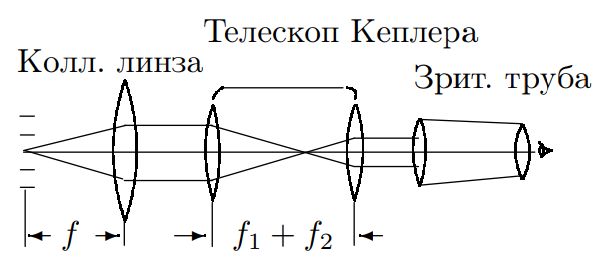
\includegraphics[scale=0.7]{kepler_setup.png}
    \caption{Телескоп Кеплера}
    \label{img:setup_kepler}
\end{figure}

Получим экспериментальное значение увеличения трубы Кеплера. Пусть $h_1$ -- размер ячейки сетки без телескопа, $h_2$ -- с телескопом. 

\begin{center}
    $h_1 = 10$ дел., \hspace{1cm} $h_2 = 27$ дел.
\end{center}

Таким образом, получим:
\begin{equation*}
    {\gamma_{K}}_{эксп} = -\frac{h_2}{h_1} = -2.7
\end{equation*}

Сравним это значение с расчитанными по формуле \eqref{eq:kep_gamma_by_focuses_diams}.

Во-первых, по диаметру оправы объектива и диаметру изображения этой оправы в окуляре:
\begin{center}
	$D_1 = 3.6 $ см, \hspace{1cm} $D_2 = 9.6 $ см
\end{center}

\begin{equation*}
    {\gamma_{K}}_{диам} = -\frac{D_2}{D_1} = -2.66
\end{equation*}

И, во-вторых, по фокусным расстояниям линз:
\begin{center}
	$f_2 = 10.6$ см, \hspace{1cm} $f_4 = 28.1$ см
\end{center}

\begin{equation*}
    {\gamma_{K}}_{фокус} = -\frac{f_4}{f_2} = -2.65
\end{equation*}

\point Теперь смоделируем трубу Галилея. Труба Галлилея получается после замены собирающей линзы в трубе Кепплера рассеивающей. Таким образом, формулы для увеличения остаются те же (за исключением знака, т.к. труба Галлилея дает прямое изображение):

\begin{equation}
    \label{eq:gal_gamma_by_focuses_diams}
    \gamma_K = \frac{f_1}{f_2} = \frac{D_1}{D_2},
\end{equation}

Заменим линзу № 4 на рассеивающую линзу № 5 (с фокусным расстоянием $f_5 = 26 см.$). Измерим увеличение:

\begin{center}
    $h_1 = 10 $ дел., \hspace{1cm} $h_2 = 25 $ дел. \par
\end{center}

\begin{equation*}
    {\gamma_G}_{эксп} = \frac{h_2}{h_1} = 2.5
\end{equation*}

Теперь сравним значение с расчитанным по формуле \eqref{eq:gal_gamma_by_focuses_diams}:

\begin{center}
    $ {\gamma_G}_{фокус} = \frac{f_4}{f_2} = 2.45 $
\end{center}

\point Моделирование микроскопа. Схема микроскопа приведена на рисунке \ref{img:setup_micro}. Увеличение микроскопа вычисляется по следующей формуле

\begin{equation}
    \gamma_M = \Gamma_{ob} \Gamma_{oc} = -\frac{\triangle}{f_1} \frac{L}{f_2},
    \label{eq:gamma_miro}
\end{equation}

где $f_1$ и $f_2$ - фокусные расстояния линз микроскопа, $\triangle = l_{12}-f_1-f_2$ см - интервал, $ l_{12} $ -- длина тубуса, $L$ - расстояние наилучшего зрения ($L = 25$ см).

\begin{figure}[h]
    \centering
    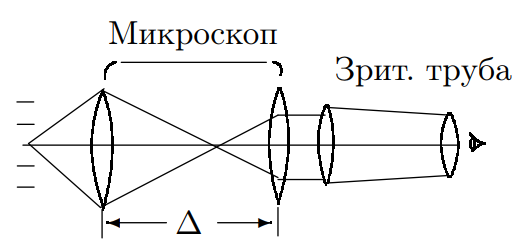
\includegraphics[scale=0.7]{micro_setup.png}
    \caption{Схема микроскопа}
    \label{img:setup_micro}
\end{figure} 

Соберем микроском с пятикратным увеличением. Для сборки используем линзы №1 ($f_1 = 7.5~ см$) и №2 ($f_2 = 10.6~ см$). По формуле \eqref{eq:gamma_miro} расчитаем необходимую длину тубуса: $l_{12} = 33.75 см.$

Измерим размер ячейки миллиметровой сетки, и расчитаем увеличение.
\begin{center}
    $h_1 = 10 $ дел., \hspace{1cm} $h_2 = 38 $ дел. \par
\end{center}

\begin{equation*}
    {\gamma_M}_{эксп} = -\frac{h_2L}{h_1f} = -4.92
\end{equation*}

где $f$ -- фокусное расстояние линзы-коллиматора $ f = f_3 = 19.3 $ см.


\parag {Заключение} ~\\
В ходе выполнения лабораторной работы были получены следующие результаты:
\begin{enumerate}
    \item Для трубы Кепплера:
        \begin{enumerate}
            \item ${\gamma_K}_{эксп.} = -2.7$
            \item ${\gamma_{K}}_{диам.} = -2.66$
            \item ${\gamma_{K}}_{фокус.} = -2.65$
        \end{enumerate}
    \item Для трубы Галлилея:
            \begin{enumerate}
                \item ${\gamma_G}_{эксп.} = 2.5 $
                \item $ {\gamma_G}_{фокус.} = 2.45 $
            \end{enumerate}
    \item Для микроскопа:
        \begin{enumerate}
            \item ${\gamma_M}_{эксп.} = -4.92 $
            \item $ {\gamma_M}_{теор.} = -5 $
        \end{enumerate}
\end{enumerate}

Как видно, значения хорошо соответствуют друг другу. Небольшое расхождение можно объяснить небольшими продольными сдвигами приборов при выставлении их на оптической скамье. 

\end{document}
 